\documentclass[a4paper,11pt,titlepage]{book}
%\usepackage{filecontents}
%\usepackage[style=authoryear,backend=bibtex]{biblatex}
% Necesario para poder hacer funcionar la bibliografia hecha en BibTeX

\usepackage{./estilos/estiloBase} % Basicamente son todas las
                                  % librerias usadas. En caso de que
                                  % falten librerias se van añadiendo
                                  % al fichero.
\usepackage{./estilos/colores}  % Algunos colores ya generados, para
                                % los algunos estilos más avanzados.
\usepackage{./estilos/comandos} % Algunos comandos personalizados

\graphicspath{{./imagenes/}} % Indicamos la ruta donde se encuentran
                             % las imagenes, para ahorrarnos la ruta
                             % completa, y solo modificar aquí si en
                             % un momento dado lo movemos
%\ifnum \@itemdepth >4\@toodeep\else
%---------------------------------------------------------------------------------

\title{{\Huge \bf 1812: La aventura}\\{\large \em Documento de diseño}\\{\normalsize Versión 0.1}}
\author{Alicia Guardeño Albertos}
\date{\today}

\begin{document}


% Renombramos las figuras y las tablas
\renewcommand{\figurename}{Figura}
\renewcommand{\listfigurename}{Indice de figuras}
\renewcommand{\tablename}{Tabla}
\renewcommand{\listtablename}{Indice de tablas}

\vfill
\maketitle
\vfill
%\newpage
%\frontmatter
    \tableofcontents
    \listoffigures
    %\listoftables

\setlength{\parskip}{\baselineskip} %Lo pongo aqui para evitar el salto de línea en los índices
%\mainmatter

\newpage
\section*{Licencia} % Por ejemplo GFDL, aunque puede ser cualquiera

Este documento ha sido liberado bajo Licencia GFDL 1.3 (GNU Free
Documentation License). Se incluyen los términos de la licencia en
inglés al final del mismo. Sin embargo, las imágenes de videojuegos comerciales incluidos están sujetos a copyright y no se distribuyen bajo licencia libre.\\

Copyright (c) 2014 Alicia Guardeño Albertos.\\

Permission is granted to copy, distribute and/or modify this document under the
terms of the GNU Free Documentation License, Version 1.3 or any later version
published by the Free Software Foundation; with no Invariant Sections, no
Front-Cover Texts, and no Back-Cover Texts. A copy of the license is included in
the section entitled "GNU Free Documentation License".\\

\newpage
\chapter{Historial de cambios}
\label{chap:historial}
En este capítulo se informará de todas las modificaciones que ha sufrido este documento, indicando la fecha y una descripción de los cambios más destacados.

\begin{itemize}
	\item \emph{20 de junio de 2014}: Primera versión del Documento de Diseño de \nombrejuego.
\end{itemize}

%\newpage
\chapter{Introducción}%Game overview
\label{chap:introduccion}
Este es el documento de diseño de \nombrejuego. El cual es un videojuego en 2D del género de las aventuras gráficas, con una ambientación en la Cádiz actual cuyo objetivo es tanto de entretener al jugador como que aprenda anécdotas y hechos relacionados con Cádiz en los años que fue asediada y vieron nacer la Constitución de 1812.

    \section{Concepto del videojuego}
        \nombrejuego es un videojuego en el que controlaremos a un estudiante de la Licenciatura de Historia de la Universidad de Cádiz, que recientemente ha suspendido un examen y va al despacho a pedir una revisión para su nota. Sin embargo, no logra encontrar al profesor y se embarcará en una aventura para descubrir el paradero de dicho profesor ayudándose de las pistas obtenidas al resolver puzzles, teniendo estos siempre una relación con la Cádiz de 1812. El videojuego tiene que estar completamente documentado, pues una gran gran parte de la jugabilidad y de la parte educativa del juego, recae completamente en el buen diseño que se haga de los puzzles, estancias e interacciones con otros personajes no controlables.
        
    \section{Género}
        \nombrejuego pretende seguir el patrón de las aventuras gráficas antiguas. Dicho género basa sus mecánicas en ir avanzando por el mundo, escenario o juego a través de la resolución de diversos puzzles, planteados como situaciones que se suceden en la historia, interactuando con personajes y objetos a través de un menú de acciones o interfaz similar, utilizando un cursor para manejar al personaje y realizar las distintas acciones.
        
    \section{Propósito y público objetivo}
        El principal objetivo de \nombrejuego es de proporcionar documentación en español sobre el diseño de videojuegos, y más específicamente en el campo de las aventuras gráficas con el documento de diseño de puzzles. También el de promocionar la historia de Cádiz. Finalmente, realizar el videojuego a partir de los diseños, poniendo a disposición de la gente el código documentado del juego y así promocionar el desarrollo organizado para proyectos con una mediana envergadura. No obstante, debe de ser un producto que sea jugable y ameno para que este desarrollo haya cumplido con sus objetivos.
        
        \nombrejuego está dirigido a todas las edades a partir de los seis años, pero principalmente a los jóvenes por ser un videojuego sencillo y tratado con un humor más juvenil. 
        
    \section{Resumen del flujo de juego}%Game flow summary
        Si bien el videojuego va a ser 2D, el movimiento del personaje dentro de los escenarios (dentro de las zonas donde se pueda caminar) será de arriba y abajo, derecha e izquierda y en diagonales. Luego para moverse entre los escenarios, se hará uso de un mapa con las localizaciones marcadas. Para poder avanzar en el juego será necesario resolver puzzles en los escenarios para poder acceder a nuevas localizaciones en el mapa.
        
    \section{Estilo visual}
    \nombrejuego tendrá un estilo sencillo, sin ser demasiado detallista para encajar con su carácter amigable y accesible. El estilo visual que más encaja sería el de las aventuras gráficas antiguas, las cuales eran gráficos pixelados asemejando a dibujos animados o cómics. Los personajes y escenarios serán caricaturescos, con colores vivos y trazos simples. En el caso de los escenarios, estos estarán basados en sitios reales a los que se les habrá simplificado o modificado para encajar con el estilo visual del videojuego.
        
    \section{Alcance del proyecto}%Project scope
    El objetivo principal es desarrollar un sistema de juego sólido, al que podamos ir añadiéndole contenidos sin apenas dificultad. En primera instancia el juego contará con nueve escenarios distintos, cada uno con uno o dos puzzles. Cada escenario representará un lugar distinto de Cádiz, y por consiguiente con una temática distinta tanto visualmente como en el problema histórico a tratar en el puzzle.
    
        \subsection{Número de niveles}
        En un principio son nueve niveles, pero este número puede variar con facilidad.
        
        \subsection{Número de Personajes No Jugables (PNJ o NPC en inglés)}
        Por ahora el número de PNJs definidos son unos cinco.
        
        \subsection{Número de puzzles}
        En un principio son diez puzzles, incluyendo un puzzle final que haga un repaso de todos las anécdotas históricas relatadas en el videojuego.


%\newpage        
\chapter{Jugabilidad y mecánicas}
\label{chap:jugabilidad}
En esta sección entraremos más en detalle en lo que a las mecánicas de \nombrejuego se refiere. Se comentarán todas las características que forman parte de la jugabilidad, y se detallarán las acciones que podrá llevar a cabo el jugador dentro de una partida típica. Además de explicar de forma concisa la organización de los menús y su utilidad.

    \section{Jugabilidad}
        \subsection{Progresión del juego}
        La progresión del juego va definida por el número de localizaciones (nuevos escenarios) desbloqueados. Al principio solo contaremos con una única localización e iremos desbloqueando las demás según resolvamos puzzles.
        
        \subsection{Progresión de la dificultad}%Challenge Structure
        %Si bien los puzzles seguirán distintos métodos para su resolución, todos los puzzles serán presentados previamente por un personaje (sea el protagonista o un PNJ).
        Cada puzzle del juego tendrán distintos métodos de resolución, ya sea uno de colocar figuras en el mapa, otro de identificación de cuadros, uno de obtener objetos, etc. Aparte de eso, la dificultad irá en aumento por la cantidad de acciones, objetos necesarios, o áreas para visitar para la resolución de dicho puzzle.
        
        \subsection{Objetivos}
        El objetivo del juego es resolver el misterio del paradero del profesor desaparecido, y por consiguiente, que el protagonista apruebe el examen suspendido. Para ello, tendrá que resolver los puzzles, uno a uno, y finalmente resolver un pequeño cuestionario con las anécdotas históricas de cada puzzle.
        
        \subsection{Flujo de juego}%Play flow
        A lo largo de esta sección, se detallará el transcurso de una partida típica a \nombrejuego. Se comentarán los pasos que ha de seguir el \emph{Jugador} desde el arranque del juego hasta completar un puzzle y pasar al siguiente nivel. De esta forma, desentrañamos el funcionamiento exacto del juego. Más adelante se definen las mecánicas y el contenido de cada pantalla.
        
        El \emph{Jugador} inicia \nombrejuego y se le presenta el \emph{Menú Principal}. Si desea iniciar una partida el \emph{Jugador} seleccionará la opción \emph{Partida nueva}, o en el caso de tener una partida ya guardada, a la opción \emph{Cargar partida} (para saber más de los menús, véase la sección ~\ref{sec:diagrama-flujo-menus}).
        
        Una vez dentro del juego, veremos al personaje principal en un escenario. Dentro del cual, podremos interactuar con el escenario haciendo \emph{clicks} para ver o interactuar con sus elementos: ver lo que son, hablar con otros personajes, coger objetos, etc. Si estamos al inicio de un escenario nuevo, se sucederá una escena cinemática (de forma en la que el protagonista se mueva y hable sin requerir ninguna acción por parte del \emph{Jugador}), y un personaje de dicho escenario nos planteará un puzzle a resolver si queremos recibir una pista sobre el paradero del profesor. Según cómo hagamos dichas interacciones resolveremos el puzzle a resolver en dicho escenario y obtendremos un nuevo escenario a donde ir.
    
    %\newpage    
    \section{Controles}
        
        \begin{figure}[H] 
			\begin{center}
				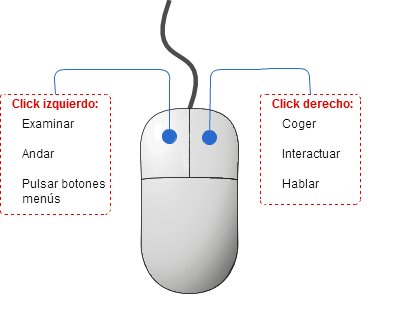
\includegraphics[scale=0.5]{controles.png}
			\end{center}
			\caption{Controles del juego}
			\label{fig:controles}
		\end{figure}
    
    %\newpage    
    \section{Mecánicas}
        
        \subsection{Movimiento}
        En esta sección definiremos cómo se moverá el personaje principal que maneja el \emph{Jugador}, además de otros movimientos tales como trasladar un objeto de sitio.
            
            \subsubsection{Movimiento general}
            Para el movimiento general del personaje principal, el jugador solo se limitará en hacer click en alguna zona donde no haya obstáculos o encima de un objeto que se pueda examinar, de forma que el personaje principal se acerque para examinarlo más detenidamente.
            
            \subsubsection{Otros movimientos}
            Los otros personajes, no se moverán o simplemente se moverán unos pasos, siento su ruta únicamente una línea recta de escasa distancia.
            
        \subsection{Objetos}
        En los escenarios en los que transcurre el juego, habrá varios objetos con los que el \emph{Jugador} podrá interactuar con ellos.
            
            \subsubsection{Describiendo objetos}
            Al mover el ratón por la pantalla, el icono del ratón cambiará a otro si está encima de un objeto. Si el \emph{Jugador} pulsa \emph{click} izquierdo, el protagonista se moverá hasta la posición más cercana a dicho objeto y le explicará al \emph{Jugador} qué es y sus impresiones propias sobre él.
            
            \subsubsection{Cogiendo objetos}
            Si el objeto es adquirible por nuestro protagonista, de la misma manera que pasamos el ratón sobre el objeto y cambia el icono del ratón al estar sobre un  objeto, en este caso hacemos \emph{click} derecho. De esta manera el protagonista se moverá hasta la posición más cercana a dicho objeto y lo cogerá, seguido de un sonido que indique el haber metido el objeto en el inventario.
            
            \subsubsection{Moviendo objetos}
            En \nombrejuego realmente no podremos mover \emph{in situ} los objetos dentro del escenario. Para poder moverlos, primero tendremos que introducir el objeto en el inventario, luego seleccionarlo dentro del inventario con \emph{click} izquierdo, y finalmente usar el objeto en el sitio concreto del escenario donde se pueda utilizar con \emph{click} derecho.
            
        \subsection{Acciones}
        Si bien casi toda las acciones se hacen de manera similar a lo descrito en la sección anterior, existen algunas diferencias que hay que puntualizarlas. Pues no todo es simplemente describir, coger y mover objetos en \nombrejuego.
        
            \subsubsection{Interruptores y botones}
            Para accionar un interruptor o botón, simplemente hay que posicionar el ratón sobre él y ver cómo cambiar el icono de este. Estando así, simplemente hay que hacer \emph{click} derecho con el ratón, el protagonista se moverá hasta donde está el interruptor o botón y lo accionará. De manera opcional, el protagonista puede decirnos si ha pasado algo en concreto al accionarlo.
            
            \subsubsection{Coger, llevar y soltar}
            En \nombrejuego solo podremos coger, llevar objetos de la manera especificada en la sección de Objetos. Soltar los objetos no será posible hasta que se hayan usado en el puzzle que los requiera.
            
            \subsubsection{Hablar}
            En el juego, podremos hablar con los otros personajes que se encuentren en el escenario. Para ello, tendremos que posicionar el ratón encima de un personaje. El icono cambiará como en las veces citadas anteriormente, y tendremos que hacer \emph{click} izquierdo. Así el protagonista se moverá a la posición más cercana que se sitúe al frente del personaje y aparecerá un diálogo entre ellos.
            
            \subsubsection{Leer}
            En \nombrejuego habrá libros y carteles para leer. La mecánica es la misma que se usa para describir un objeto, dado que los libros y carteles son objetos. 
         
	%\newpage
	\section{Inteligencia Artificial}
	En la mayoría de los videojuegos es uno de los puntos más importante, pues ella rige el comportamiento de todos los personajes, e incluso de objetos. Un enemigo que sigue una ruta y te persiga si te ve, un semáforo que cambia de luces y los coches se mueven con ello, todo esto y mucho más es gracias a las inteligencia artificial. Existen muchos y variados algoritmos para realizar distintos comportamientos dependiendo de si buscas que un personaje haga una ruta, una estrategia, o que actúen a modo de colmena los personajes que aparecen el juego, y más aún que desconozco. Sin embargo, en las aventuras gráficas no se suele hacer un gran uso de estas pues los personajes no suelen moverse de su sitio, y las conversaciones son lineales. Pero si hay un punto que a veces usa una inteligencia artificial, cuando queremos que el personaje que lleva el \emph{Jugador} se mueva en un escenario con obstáculos.
        
            \subsection{Cálculo de la ruta del movimiento del personaje principal}
             Cuando el \emph{Jugador} quiera mover al personaje principal y haga \emph{click} en el escenario para ello. Pueden pasar varias cosas según la distancia que hay entre el punto al que el \emph{Jugador} quiere ir, y si hay obstáculos en el camino para llegar a ese punto.
             
             Si la distancia fuera corta, en línea recta y sin obstáculos, el movimiento se calcularía como una línea recta directa.
             
             En el caso de que hubiera obstáculos pero fuera posible llegar desde una ruta que no sea en línea recta, el personaje principal seguirá una ruta realizada con un algoritmo A\* o similar. De esta manera calcula la ruta más corta desde donde esta nuestro personaje principal hasta el punto donde queremos llevarlo, y finalmente lo ejecuta para llevar a cabo el movimiento.
            
            \subsection{Personajes No Jugables (PNJs) o \emph{Non Player Characters} (NPCs)}
        	Si algunas veces en las aventuras gráficas aparecen PNJs enemigos que persiguen al Protagonista o amistosos que estén dando vueltas por una ruta prefijada, en el caso de \nombrejuego no va a ser así. Los PNJs se quedarán en un sitio prefijado sin moverse y solo interactuarán con el Protagonista para iniciar una conversación. 
            
	%\newpage
	    \section{Físicas}
	    El juego poseerá físicas en 2D, osease, colisiones entre planos. De esta manera, el jugador solo podrá mover su personaje sobre ciertas áreas, saber cuándo estamos pulsando encima de un objeto o personaje con el que podemos interactuar, poder acceder al menú gracias a un menú gráfico, etc. No poseerá elementos gravitacionales y toda colisión tendrá valores discretos (no analógicos) para indicar si se ha producido una colisión o no.
	    
	    	\subsection{Sistema de colisiones}
	    	El sistema de colisiones será por cajas poligonales, en las que al colisionar unas con otras no podrán atravesarse mutuamente. Los elementos del juego que poseerán una caja de colisiones son:
	    	
	    	\begin{itemize}
	    	\item \negrita{Personaje principal:} Tendrá una caja de colisión en la parte inferior del \emph{sprite}. Esto es debido a que la parte superior de este puede superponerse parcialmente a un objeto que posea una caja de colisión y esté situado en un plano de fondo. Un ejemplo para esclarecer esto: el personaje principal puede estar encima de una pared parcialmente, pero sus pies no para evitar que camine sobre ella. A su vez el protagonista no podrá atravesar elementos en primer plano bajo ningún concepto, pero si puede aparecer detrás de ellos.
	    	\item \negrita{PNJs:} Su caja de colisión será idéntica a la del personaje principal. Pero esta servirá para que cuando el ratón se ponga encima del PNJ, el sistema lo detectará y contará como que el personaje principal puede hablar con dicho PNJ. El icono del ratón cambiará para mostrar que se puede realizar dicha acción.
	    	\item \negrita{Objetos:} Los objetos tendrán otra caja de colisión que no podrá atravesarse, pero esta estará más enfocada a que colisione con el ratón. Pues cuando este se ponga encima del objeto, se detectará la colisión y contará como que se puede examinar o interactuar con dicho objeto. El icono del ratón cambiará para mostrar que se puede realizar dicha acción.
	    	\item \negrita{Obstáculos:} Poseerán cajas de colisiones en la que su única función será el de no poder ser atravesados por el personaje principal. 
	    	\end{itemize}

%\newpage            
\chapter{Interfaz}
\label{chap:interfaz}
En un videojuego, la interfaz es esencial para transmitir información al jugador tanto dentro del juego para poder interactuar con dicho mundo, como en los menús para modificar elementos externos del juego tales como guardar una partida, cambiar especificaciones de la visualización del juego, etc.Por ello, en esta sección se especificará con detalle cada una de las pantallas y los menú que componen \nombrejuego. Además, se indicarán las transiciones entre ellas así como la utilidad de cada elemento de la GUI (\emph{Graphical User Interface}). Las imágenes adjuntas son bocetos que ilustran los componentes que debe contener cada pantalla, no obstante, los artistas podrán hacer cambios en la apariencia y disposición de los elementos si así lo consideran oportuno.
    
    \section{HUD (\emph{Heads-Up Display})}
    
    \label{sec:menus}
        \section{Diagrama de flujo}
        En todo juego, los menús necesitan de una jerarquía u orden a la hora de aparecer en pantalla. Para ello, normalmente se usa un diagrama que establece de manera visual el orden y la manera de cómo se puede acceder a los distintos menús durante el juego. Normalmente en un juego pequeño, dónde normalmente solo hay uno o dos menús, se puede hacer innecesario. Pero en cuanto intentemos realizar un juego que necesite de más de cuatro menús diferentes, se hace inviable el no esquematizar el orden de estos. No solo para el programador, sino para el jugador, pues el tener que ir buscando el menú específico de forma complicada, hará que dicho jugador se canse rápidamente del juego y consecuentemente abandonarlo. El siguiente diagrama de estados muesta las pantallas presentes a lo largo de \nombrejuego y las transiciones entre ellas.
        
        \begin{figure}[H] 
                \begin{center}
                    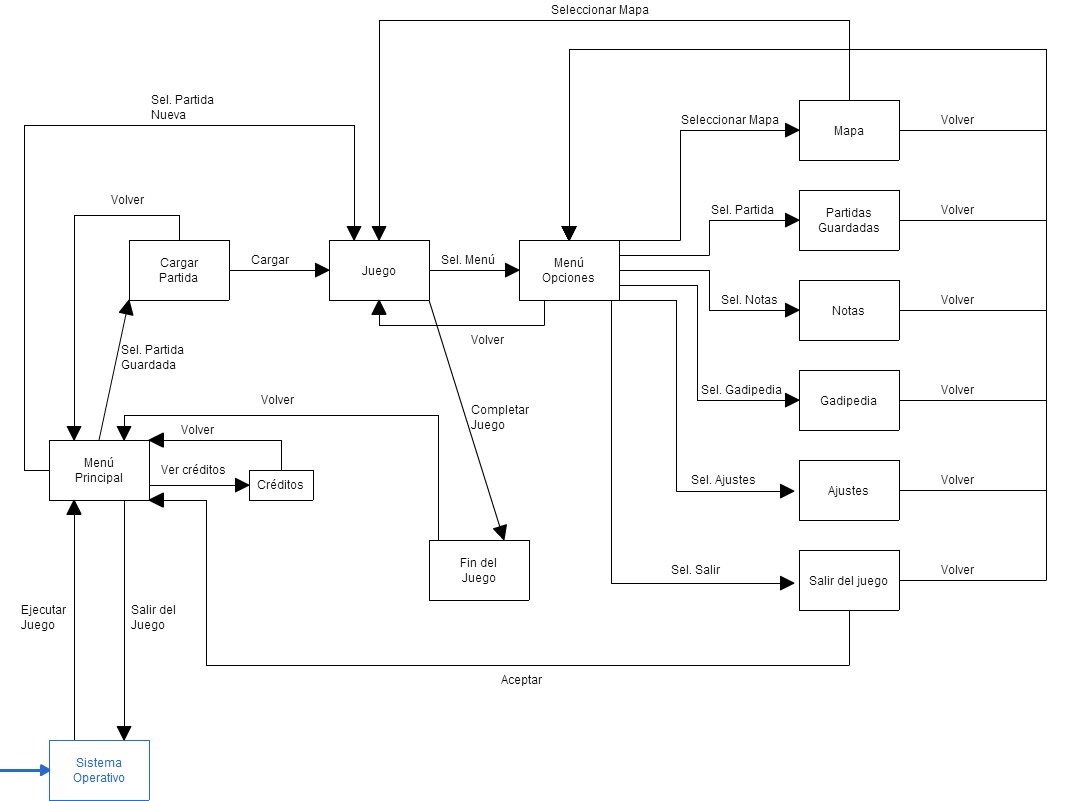
\includegraphics[scale=0.45]{diagrama_flujo_menu.png}
                \end{center}
                \caption{Diagrama de flujo de pantallas en el juego}
                \label{fig:diagrama-flujo-menu}
            \end{figure}
        
        \section{Descripciones de las pantallas}
        En esta sección nos centraremos en describir de manera individual todas las pantallas que hacen aparición en \nombrejuego.
        
        \newpage
            \subsection{Menú principal}
            A continuación el boceto de la pantalla de \emph{Menú Principal} :
            
            \begin{figure}[H] 
                \begin{center}
                    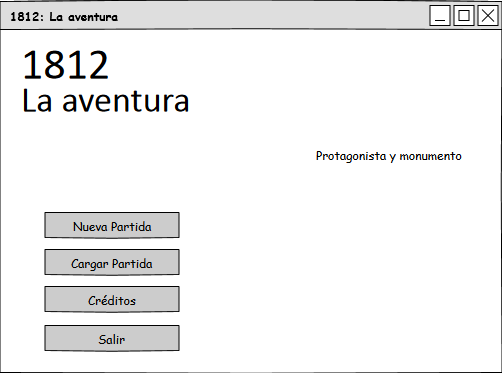
\includegraphics[scale=0.7]{men_principal.png}
                \end{center}
                \caption{Boceto del Menú Principal}
                \label{fig:menu-principal}
            \end{figure}
            
            Lista y descripción de todos sus componentes:
            \begin{itemize}
            \item \negrita{Botón Nueva Partida}: al pulsarlo lleva a la pantalla de \emph{Crear Partida}.
            \item \negrita{Botón Cargar Partida}: al pulsarlo lleva a la pantalla de \emph{Cargar Partida}.
            \item \negrita{Botón Créditos}: al pulsarlo nos lleva a la pantalla \emph{Créditos}.
            \item \negrita{Botón Salir}: al pulsarlo nos lleva de vuelta al Sistema Operativo.
            \item \negrita{Protagonista y monumento}: Una ilustración del protagonista de \nombrejuego situado en un monumento emblemático del 1812.
            \end{itemize}
            
            \newpage
            \subsection{Cargar Partida}
            A continuación el boceto de la pantalla de \emph{Cargar Partida} :
            
            \begin{figure}[H] 
                \begin{center}
                    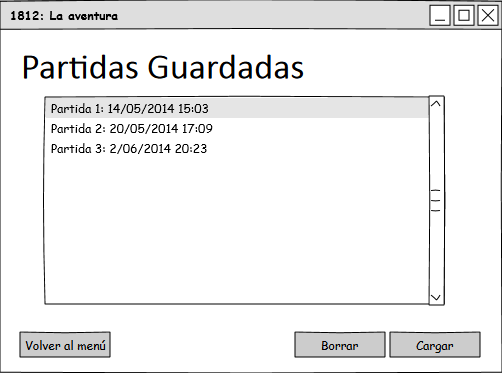
\includegraphics[scale=0.7]{cargar_partida.png}
                \end{center}
                \caption{Boceto de la pantalla de Cargar Partida}
                \label{fig:cargar-partida}
            \end{figure}
            
            Lista y descripción de todos sus componentes:
            \begin{itemize}
            \item \negrita{Lista de partidas}: lista con las partidas guardadas hasta el momento. Se muestra el día y la hora de la última actualización de esa partida.
            \item \negrita{Botón Cargar}: al pulsarlo coge la partida seleccionada y carga la pantalla de juego tal y como la dejamos.
            \item \negrita{Botón Borrar}: al pulsarlo nos dará un
            \item \negrita{Botón Volver al menú}:
            \end{itemize}
            
            \newpage
            \subsection{Créditos}
            
            
            \newpage
            \subsection{Menú Opciones}
        
        
            \newpage
            \subsection{Mapa}
            
            
            \newpage
            \subsection{Partidas guardadas dentro del juego}
            A continuación el boceto de la pantalla de \emph{Partidas Guardadas} dentro del juego :
            
            \begin{figure}[H] 
                \begin{center}
                    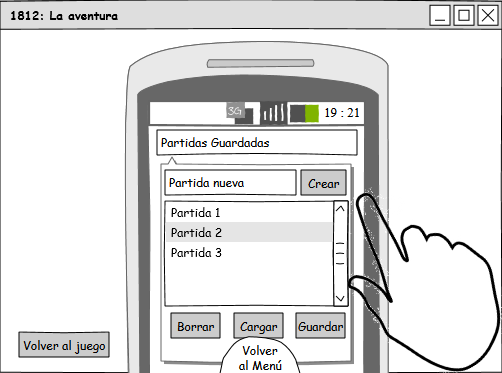
\includegraphics[scale=0.7]{cargar_partida_dentro_del_juego.png}
                \end{center}
                \caption{Boceto de la pantalla de Cargar Partida}
                \label{fig:cargar-partida-dentro-juego}
            \end{figure}
            
            Lista y descripción de todos sus componentes:
            \begin{itemize}
            \item \negrita{Crear partida nueva}: etiqueta y caja de texto para introducir el nombre de la nueva partida.
            \item \negrita{Botón Crear}: crea una nueva partida con el nombre que contiene la caja de texto. Si el perfil existe o no se ha introducido un nombre, una ventana con un mensaje aparecerá indicando el error.
            \item \negrita{Lista de partidas}: lista con las partidas guardadas hasta el momento. Se muestra el día y la hora de la última actualización de esa partida.
            \end{itemize}
            
            \newpage
            \subsection{Gadipedia}
            
            
            \newpage
            \subsection{Notas}
            
            
            \newpage
            \subsection{Ajustes}
            
            
            \newpage
            \subsection{Salir}
        %\subsection{Trucos y \emph{Easter Eggs}}
        %Por ahora no hay intención de introducir trucos y \emph{Easter Eggs}.

%\newpage        
\chapter{Argumento y personajes}%Story Setting and Character
\label{chap:argumento}
En este apartado detallaremos el argumento y el guión del juego. Al ser \nombrejuego un videojuego del género de las aventuras gráficas, estos tienen más importancia, pues a través de la narración vamos conociendo a los personajes y a cómo resolver los puzzles que nos deparará en el juego. 
    \section{Argumento y narrativa}
        \subsection{Trasfondo argumental}
        Hace un par de días, el Protagonista ha suspendido un examen con la infame nota de un 4,9. Ante tal nota, el Protagonista se dispone ir a la revisión del examen al despacho del profesor. Lamentablemente el profesor no se encuentra allí, pero cómo nuestro Protagonista es un cabezota, hará todo lo posible para encontrar al profesor y convencerle de que merece el aprobado.
        
        \subsection{Elementos clave}
        \subsection{Secuencias cinemáticas}
        En esta sección detallaremos las secuencias cinemáticas que habrá en \nombrejuego. Estos son momentos del juego en el que el \emph{Jugador} no podrá controlar al Protagonista y el juego tomará control de la situación. En juegos grandes se suele invertir una cantidad enorme en hacer las secuencias cinemáticas lo más vistosas posibles empleando en su mayoría vídeos. Juegos más pequeños prefieren evitar estas escenas por el enorme gasto que suponen, y se las ingenian en hacerlos de otras maneras.
        
        En \nombrejuego al ser también un juego de pequeña envergadura, la cantidad de secuencias cinemáticas del juego es mínima y sólo habrá una al principio de entrar en un nuevo escenario, y otra después de resolver un puzzle. Por ahora solo hay 
            
    \section{Mundo del juego}
        \subsection{Estilo visual general}%General Look and Feel
        \subsection{Primer escenario}
        \subsection{Segundo escenario}
        %...
        
    \section{Personajes}
    En esta sección definiremos brevemente a los personajes que intervendrán en el juego. Servirá sobretodo a la hora de definir las personalidades y reflejarlas en la manera de hablar de estos en el guión.
    
        \subsection{Protagonista}
            \subsubsection{Trasfondo}
            Estudiante del Grado de Historia en la Universidad de Cádiz, ha suspendido un examen con un 4,9 y hará todo lo posible para convencer al profesor de que merece el aprobado.
            \subsubsection{Personalidad}
            De personalidad humorística y despreocupada, con cierta aversión al profesor que le ha suspendido.
            \subsubsection{Aspecto}
            Pelo negro y desaliñado, con barbita dejada tal y cómo se lleva ahora entre los universitarios. Con sudadera y vaqueros.
                
        \subsection{Profesor}
            \subsubsection{Trasfondo}
            Profesor de una asignatura en el Grado de Historia en la Universidad de Cádiz, no se sabe donde está.
            \subsubsection{Personalidad}
            Despistado y afable, pero es muy estricto con los alumnos.
            \subsubsection{Aspecto}
            Típico profesor mayor con barba y traje.
            
        \subsection{Bibliotecaria}
            \subsubsection{Trasfondo}
            Es la bibliotecaria de la Facultad de Filosofía y Letras desde hace muchos años, ya los años les pasa factura y se olvida de las cosas o no puede llevar los libros con tanta facilidad.
            \subsubsection{Personalidad}
            Olvidadiza y muy estricta con las normas de la biblioteca, sobretodo con la de mantener el silencio.
            \subsubsection{Aspecto}
            Mujer mayor con gafas de lectura antigua.
    
    Estos son los personajes definidos por ahora, más adelante se irán añadiendo más y así sucesivamente hasta completar con todo el elenco de personajes que harán su aparición en el juego.
        %...

%\newpage        
\chapter{Niveles}
\label{chap:niveles}
%Los niveles en este juego, serán los distintos escenarios donde el Jugador pueda moverse. \nombrejuego tiene pocos niveles por las limitaciones de tiempo y dinero que implica hacer un proyecto final para una carrera universitaria, pero todos estos están esquematizados para esclarecer todo lo que contiene y sucede dentro de dicho nivel.

Los niveles son los distintos escenarios por los que un \emph{Jugador} tendrá que pasar para poder avanzar en el videojuego, de forma que \negrita{siempre} hay que resolver el problema que nos supone el nivel actual para poder llegar al siguiente, y así sucesivamente hasta que acabemos el juego. Estos niveles o escenarios pueden ser pantallas estáticas tales como un nivel del Tetris, o un escenario donde el \emph{Jugador} pueda moverse de un lado para otro. En este segundo caso pueden existir dos variantes, que el \emph{Jugador} pueda recorrer el nivel con una vista en primera persona, o en tercera persona teniendo el \emph{Jugador} que mover un personaje para recorrerlo.

En cualquier caso, el diseño de los niveles es \negrita{vital} para que el jugador disfrute de la experiencia de superar el videojuego en concreto que vayamos a crear. Hay que lograr que nunca haya momentos aburridos y a su vez que no haya demasiados momentos de tensión que acaben en frustración para el \emph{Jugador}, y que acaben consiguiendo que este lo deje y nunca termine el juego. De hecho, aunque un juego pueda poseer buenas e interesantes mecánicas, los \emph{Jugadores} no las verán hasta que entren en juego en algún nivel e interactuen con este.

%En el caso de aventuras gráficas, concretamente \nombrejuego que es el juego a desarrollar aquí, sus niveles van divididos en distintos escenarios a recorrer. En estos hay que buscar objetos o sitios donde poder interactuar con el escenario u otros personajes, de forma que si hacemos la combinación correcta, logramos resolver el problema que nos han propuesto y así seguir avanzando hacia nuestro objetivo. En resumen: 

En el caso de aventuras gráficas, concretamente \nombrejuego que es el juego a desarrollar aquí, sus niveles van divididos en distintos escenarios a recorrer. De forma concisa, estos son los pasos que hay que seguir en el diseño de los niveles en este tipo de género:

\begin{enumerate}
	\item Al inicio del juego, nos plantean en el argumento un problema u objetivo a conseguir.
	\item Para poder conseguir el objetivo principal, hay que dividirlo en distintos sub-objetivos.
	\item Cada sub-objetivo se resuelven con la combinación de acciones y objetos adecuadas.
	\item Una vez resuelto dicho sub-objetivo, obtenemos nuevos niveles o escenarios a visitar.
	\item En los escenarios nuevos nos proporcionarán un nuevo sub-objetivo que nos acercará al objetivo principal del videojuego.
	\item Se repite el proceso de sub-objetivos hasta que finalmente recompensa a los \emph{Jugadores} con la obtención del objetivo principal del juego.
\end{enumerate}

Como véis, en las aventuras gráficas, muchas veces hablar de puzzles es sinónimo de hablar de niveles. En un principio, en \nombrejuego se tomó la decisión inicial de separar la parte de los puzzes (niveles) en otro documento mejor organizado. No se descarta en un futuro incluir dicha parte en este documento, pero para la versión del documento de diseño que nos ocupa, este capítulo sólo se quedará como orientativo. 

Las secciones siguientes se explicarán de forma breve cuál es su propósito en el juego, y de cómo podríamos escribirlas.


    \section{Nivel 1}
    Este es el nivel donde comenzamos el juego. Suele ser más simple y largo que otros, pues se usa principalmente para explicarle al \emph{Jugador} de qué va el juego y cuál es el objetivo principal de este, además de proporcional diversos elementos con los que el \emph{Jugador} empiece a familiarizarse con las mecánicas básicas del juego. 
        \subsection{Sinopsis}
        Aquí vendría un resumen de lo que va a pasar en este nivel, de sus características y elementos más destacados.
        \subsection{Introducción}
        Aquí deberíamos escribir qué es lo que ha sucedido antes de empezar el nivel y los hechos que pueden influir en el transcurso de este.  
        \subsection{Objetivos}
        Esto es lo antes comentado con los sub-objetivos del juego, aquí hay que decir qué es lo que el \emph{Jugador} tiene que lograr hacer en este nivel.
        \subsection{Descripción física}
        Tal y como indica el nombre, aquí incluiríamos una descripción detallada del nivel y de sus elementos.
        \subsection{Mapa}
        En el caso de que el nivel fuera de gran extensión, o que el nivel perteneciera a un lugar concreto dentro del mundo en el que se va a desarrollar el juego, se tendrían que incluir aquí imágenes diversas explicando los puntos de referencia o elementos clave del nivel. Así tanto para que el que se encarga de diseñar los niveles tenga claro donde colocar los elementos dentro del nivel, como para que el \emph{Jugador} tenga puntos de referencia para orientarse dentro del nivel.
        \subsection{Camino crítico}
        En los niveles, pueden haber distintas maneras de obtener los elementos clave para conseguir el objetivo del nivel. Aquí habría que detallar todas las rutas diferentes que un \emph{Jugador} puede seguir a través del nivel para conseguir el objetivo. Aunque hay que puntualizar, que a veces las rutas de resolución de un nivel pueden ser casi infinitas, en ese caso, solo tendríamos que escribir aquí las rutas principales que usará la mayoría de \emph{Jugadores}. 
        \subsection{Resolución del nivel}
        Aquí, a modo de guía de resolución de juego, tenemos que explicar cómo se resuelve el problema que nos presenta el nivel para lograr el objetivo.
        \subsection{Conclusión}
        Aquí comentaremos los sucesos que ocurran una vez finalizado el nivel y antes de que comience el siguiente.
        
    %\section{Nivel 2}
    %...

%%\newpage
%\chapter{Interfaz}
%
%    \section{Sistema visual}
%        \subsection{HUD}
%        \subsection{Menús}
%        
%    \section{Controles del sistema}
%        
%        \section{Audio}
%        \subsection{Música}
%        \subsection{Efectos de sonido}
%

%\newpage
%\chapter{Inteligencia Artificial}

%    \section{ \emph{Non Player Characters} (NPCs)}
        
%    \section{Jugador y sistema de colisiones}


        
%\newpage
\chapter{Apartado técnico}
\label{chap:tecnico}
En este apartado detallaremos las partes relacionadas con el desarrollo del videojuego como software, tales como para qué plataforma se va a desarrollar, y cómo y con qué se va a desarrollar \nombrejuego.

    \section{Hardware objetivo}
    \nombrejuego al ser una aventura gráfica, estará enfocado principalmente al PC. Tendrá que ser jugado con teclado y ratón. Sin embargo, si hubiera tiempo durante el desarrollo, no se descarta una conversión a Android.
    
    \section{Hardware y Software de desarrollo}
    Algunas veces, pueden ocurrir incidencias debido a las peculiaridades del hardware y software concretos con el que se desarrolla un juego. Por lo tanto, siempre es recomendable escribir las especificaciones tanto de hardware como de software en los que se desarrollan los videojuegos. En este caso, \nombrejuego se desarrollará en un PC con las siguientes especificaciones técnicas:
    
    \begin{itemize}
    \item Procesador: Intel(R) Core(TM) i7-2700K CPU @ 3.50GHz (8 CPUs), ~3.5GHz
    \item Memoria: 16384 MB RAM
    \item Tarjeta Gráfica: NVIDIA GeForce GTX 570 1GB
    \item Sistema Operativo: Windows 7 Enterprise 64 bis (6.1, compilación 7601)
    \end{itemize}
    
    \section{Procedimientos y estándares de desarrollo}
    Un proceso para el desarrollo de software, también denominado ciclo de vida del desarrollo de software es una estructura aplicada al desarrollo de un producto de software, en este caso un videojuego. Hay varios modelos a seguir para el establecimiento de un proceso para el desarrollo de software, cada uno de los cuales describe un enfoque diferente para diferentes actividades que tienen lugar durante el proceso. 
    
    En el caso de \nombrejuego, el proceso que se va a seguir es el de Modelo de desarrollo en Cascada. Este modelo se caracteriza en que se ordenan las etapas del proceso para el desarrollo de software, de tal forma que el inicio de cada etapa debe esperar a la finalización de la etapa anterior. Al final de cada etapa, el modelo está diseñado para llevar a cabo una revisión final, que se encarga de determinar si el proyecto está listo para avanzar a la siguiente fase.
    
    Las etapas son las siguientes:
    \begin{enumerate}
    \item \negrita{Análisis}: En esta fase se analizan las necesidades de los usuarios finales del software para determinar qué objetivos debe cubrir. De esta fase surge una memoria llamada documento de especificación de requisitos, que contiene la especificación completa de lo que debe hacer el sistema sin entrar en detalles internos.
Es importante señalar que en esta etapa se debe consensuar todo lo que se requiere del sistema y será aquello lo que seguirá en las siguientes etapas, no pudiéndose requerir nuevos resultados a mitad del proceso de elaboración del software de una manera.
    
    \item \negrita{Diseño}: Descompone y organiza el sistema en elementos que puedan elaborarse por separado, aprovechando las ventajas del desarrollo en equipo. Como resultado surge el SDD (Documento de Diseño del Software), que contiene la descripción de la estructura relacional global del sistema y la especificación de lo que debe hacer cada una de sus partes, así como la manera en que se combinan unas con otras.
Es conveniente distinguir entre diseño de alto nivel o arquitectónico y diseño detallado. El primero de ellos tiene como objetivo definir la estructura de la solución (una vez que la fase de análisis ha descrito el problema) identificando grandes módulos (conjuntos de funciones que van a estar asociadas) y sus relaciones. Con ello se define la arquitectura de la solución elegida. El segundo define los algoritmos empleados y la organización del código para comenzar la implementación.
    \item \negrita{Implementación}: Es la fase en donde se implementa el código fuente, haciendo uso de prototipos así como de pruebas y ensayos para corregir errores.
Dependiendo del lenguaje de programación y su versión se crean las bibliotecas y componentes reutilizables dentro del mismo proyecto para hacer que la programación sea un proceso mucho más rápido.

    \item \negrita{Pruebas}: Al final de la implementación, normalmente hay un proceso de verificación o de pruebas. De manera que los elementos, ya programados, se ensamblan para componer el sistema y se comprueba que funciona correctamente y que cumple con los requisitos.
    
    \item \negrita{Mantenimiento}: Una vez terminado el desarrollo del software, hay una última fase de duración indefinida que es la de mantenimiento. En esta simplemente es que durante el ciclo de vida útil del software, hay que reparar errores que se hayan pasado en la etapa de pruebas o irle añadiendo nuevas funcionalidades que el público objetivo pida y así alargar su vida útil.
    \end{enumerate}
    
    Si bien esta manera de desarrollar no puede ser la más óptima, pues en cuanto se descubra un fallo que pasó desapercibido en una etapa y haya que modificarlo, hay que invertir mucho esfuerzo y parar el desarrollo. Pero es la más sencilla para proyectos de poca envergadura y que tengan bajo coste. Además de fomentar las buenas prácticas al poner un orden a la hora del desarrollo, y hacer que pensemos cómo hacer las cosas antes de llevarlas a cabo. También es una buena opción para los proyectos que están orientados a documentos como el de \nombrejuego, por ello, este es el procedimiento de desarrollo elegido. 
    
    \section{\emph{Game Engine}}
    \programa{Unity3D} será el \emph{Game Engine} con el que se desarrollará \nombrejuego. Los motivos son porque es uno de los \emph{Game Engines} más usados en la industria del videojuego independiente por su capacidad de prototipado rápido y de bajo coste, además de ser uno de los que más gente usa para iniciarse en el mundo del desarrollo de los videojuegos. 
    
    \section{Lenguaje de programación}
    Unity3D acepta C\#, JavaScript y Boo como lenguajes de programación para sus scripts. \nombrejuego se desarrollará por C\# por sus similitudes con Java y C++, lenguajes enseñados en la carrera. Además de poseer una estructura clara para poder realizar Programación Orientada a Objetos (POO) y hacer uso de Estructuras de Datos. 


%\newpage    
\chapter{Apartado artístico}
\label{chap:artistico}
En este apartado detallaremos el estilo que deben seguir los gráficos en el juego a partir del arte conceptual, las guías de estilo, descripciones de cómo deben ser personajes y escenarios, escenas cinemáticas, etc.

    \section{Arte conceptual}
    El arte conceptual, en un videojuego, sirve para definir tanto personajes, escenarios como el estilo de los gráficos de los que va a tratar el juego. Normalmente en juegos que pretenden dar un toque distintivo mediante el apartado gráfico, ya sea por diferenciar su estilo propio o para causar determinadas emociones o ambientación, es muy importante. Pero en cambio, en juegos pequeños o que los gráficos sean más secundarios, no suelen tener tanta carga y se deja más al gusto personal del grafista. \nombrejuego un juego medianamente pequeño, su arte conceptual es escaso y se deja también en manos de la grafista. 
    %El único arte conceptual que incluiremos es el diseño inicial del Protagonista, por dar un ejemplo:
    
    \section{Guías de estilo}
    En los videojuegos siempre es necesario que haya una uniformidad en los gráficos, no sólo con el estilo visual, sino con el tamaño de los gráficos y de las pantallas. Asimismo, \nombrejuego propondrá las siguientes guías para los gráficos y que así la grafista pueda atenerse a unas normas a la hora de la realización de los gráficos. Dichas normas, son más de sugerencia para conseguir una uniformidad que una imposición hacia el grafista. Así que si la ocasión lo requiere, el grafista podría saltarse las guías siempre y cuando se consulte con los otros miembros del equipo relacionados con el arte del juego y se llegue a un consenso para ese cambio. Estas son las guías para \nombrejuego:
    
    \begin{itemize}
    \item Personajes: 64x40 píxeles de resolución original, al que luego se le aplicará un \emph{zoom} por dos veces.
    \item Escenarios: 320x240 píxeles de resolución original, al que luego se le aplicará un \emph{zoom} por dos veces.
    \item Pantalla: 1280x960 píxeles será la resolución original de la pantalla, a partir de ella se adaptará a las distintas resoluciones más comunes en los ordenadores.
    \item Objetos: 32x32 píxeles de resolución original, al que luego se le aplicará un \emph{zoom} por dos veces.
    \item Paleta de colores: preferiblemente 256 colores (8 bits) para simular mejor el ser un juego antiguo, pero si se diera el caso de necesitar más colores, no habría ninguna restricción en usarlos.
    \end{itemize}
    
    \section{Personajes}
    En esta sección haremos una pequeña descripción de los personajes que aparecen en el juego, de forma que esta sea útil para la grafista a la hora de saber cómo diseñar a estos. Los personajes por ahora son los siguientes:
    
    \begin{itemize}
    \item \negrita{Protagonista}: Un estudiante universitario con los pelos revueltos, con sudadera, vaqueros y zapatillas.
    \item \negrita{Profesor}: El típico profesor mayor de universidad, con barba y traje.
    \item \negrita{Bibliotecaria}: La típica bibliotecaria, una señora mayor con gafas de lectura colgadas en la pechera.
    \item \negrita{Escritor}: Un escritor afrancesado y borracho, sentado en la mesa de firma de sus libros.
    \item \negrita{Junta directiva}: Varios hombres sentados con traje de ejecutivo y mirada inquisitoria, sentados en una mesa larga como si fuera un juicio.
    \end{itemize}
    
    \section{Escenarios}
    En esta sección haremos una pequeña descripción de los escenarios que aparecen en el juego, de forma que esta sea útil para la grafista a la hora de saber cómo diseñar a estos. Los escenarios por ahora son los siguientes:
    
    \begin{itemize}
    \item \negrita{Pasillo de la Facultad}: Un pasillo de la Facultad con varias puertas que dan a los despachos de distintos profesores.
    \item \negrita{Despacho del profesor}: El despacho al que pertenece el profesor con el que quiere hablar el Protagonista, tiene dos mesas (son dos profesores por despacho), una estanteria con libros y otras cosas, un tablón de corcho con un mapa, carteles, etc.
    \end{itemize}
    
    Estos son los escenarios por ahora, se irán añadiendo más conforme se avance el desarrollo del juego.
    
    \section{Objetos}
    En esta sección detallaremos brevemente los objetos que el Protagonista puede llevar en el inventario. Los objetos por ahora son los siguientes:
    \begin{itemize}
    \item \negrita{Examen suspendido}: Una hoja escrita con un 4,9 en rojo.
    \item \negrita{Banderitas}: Una banderita española y varias francesas con una chincheta.
    \item \negrita{Nota de la biblioteca}: Una pequeña nota que indica que el profesor debe ir a la biblioteca.
    \end{itemize}
    
    \section{Escenas cinemáticas}
    En \nombrejuego prácticamente no hay escenas cinemáticas, pues se hará uso de las animaciones de los personajes para crear las escenas controladas por el juego. Solo habrá una escena cinemática como tal, que será el final del juego en el que se verán imágenes del Protagonista feliz por haber aprobado y el de otros personajes a modo de epílogo, mientras se muestras los créditos y los agradecimientos.
    
    \section{Miscelánea}
    En esta sección suelen entrar los gráficos que no tienen cabida en las otras secciones. Concretamente en \nombrejuego se necesitarán los siguientes gráficos extras:
    \begin{itemize}
    \item \emph{Smartphone} del Protagonista, negro y únicamente táctil.
    \item Botones de las aplicaciones del \emph{smartphone} del Protagonista.
    \item Mano del Protagonista que hace como que toca el \emph{smartphone}.
    \end{itemize}

    
%\newpage    
\chapter{Apéndice}
\label{chap:apendice}
 \section{Organización de los recursos dentro del proyecto}
    Que haya una buena organización de los recursos facilita mucho el trabajo a los desarrolladores a la hora de tener que implementarlo dentro del juego, y así no tener que buscarlo en un sinfín de carpetas desorganizadas. Por ello es importante establecer una jerarquía en el orden de los recursos y de las carpetas que lo contengan. La organización de los recursos dentro del repositorio de \nombrejuego es la siguiente:
    
    
    \begin{itemize}
    \item \negrita{Recursos}/
        \begin{itemize}
        \item Audio/
            \begin{itemize}
            \item Música/
            \item FX/
            \end{itemize}
        \item Gráficos/
            \begin{itemize}
            \item GUI/
                \begin{itemize}
                \item Pantalla 1/
                \item Pantalla 2/
                \item ...
                \end{itemize}
            \item HUD/
            \item Personajes/
                \begin{itemize}
                \item Personaje 1/
                \item Personaje 2/
                \item ...
                \end{itemize}
            \item Escenarios/
                \begin{itemize}
                \item Escenario 1/
                \item Escenario 2/
                \item ...
                \end{itemize}
            \item Objetos/
                \begin{itemize}
                \item Objeto 1/
                \item Objeto 2/
                \item ...
                \end{itemize}
            \end{itemize}
        \end{itemize}
    \end{itemize}
    
    \section{Lista de recursos}
    Aquí haremos una lista que se irá actualizando con los recursos audiovisuales necesarios para poder realizar \nombrejuego. Así no se hará ningún trabajo de más o de menos, y que en el caso de tener que realizar modificaciones, estas sean pocas.
    
        \subsection{Arte}
        Todos los recursos gráficos que necesitará el juego, por ahora son los comentados en las siguientes secciones y sub-secciones.
            \subsubsection{Lista de sprites y fondos}
            Los \emph{sprites} son el nombre con el que se llama a los dibujos pixelados con los que se hacen los gráficos 2D para los videojuegos, si bien los fondos son sprites es mejor llamarlos de manera diferente, el motivo principal es porque existe la diferencia de que un fondo y un sprite es su tamaño. Pues un fondo ocupa toda la pantalla, mientras que un sprite es mediano o pequeño, pero nunca ocupa la pantalla en su totalidad.
            Lista de sprites de personajes:
            \begin{itemize}
            \item Protagonista.
            \item Bibliotecaria.
            \item Profesor.
            \item Escritor fracasado en su mesa de firma de libros.
            \item Otro profesor.
            \item Vendedor de la tienda de recuerdos.
            \end{itemize}
            
            Lista de sprites de objetos:
            \begin{itemize}
            \item Examen con la nota de 4,9 puntos en rojo.
            \item Banderitas de España y Francia.
            \item Nota de biblioteca.
            \end{itemize}
            
            \subsubsection{Lista de animaciones}
            \begin{itemize}
            \item Protagonista caminando.
            \item Protagonista hablando.
            \item Protagonista cogiendo objeto del suelo y metiéndoselo en el bolsillo de la sudadera.
            \item Protagonista cogiendo un objeto a su nivel y metiéndoselo en el bolsillo de la sudadera.
            \item Protagonista mirando el móvil.
            \item Nota de papel cayendo en el suelo.
            \end{itemize}
            
            \subsubsection{Lista de efectos}
            En este juego no hay efectos.
            
            \subsubsection{Lista de arte de la interfaz}
            \begin{itemize}
            \item Icono de lupa para el ratón.
            \item Icono de lupa con borde blanco (u otro elemento que destaque) para indicar que hay un objeto con el que se puede interactuar.
            \item Icono de bocadillo de cómic para el ratón.
            \item Icono de flecha para cambiar o salir de escenario. 
            \item Fondo con un \emph{smartphone} negro y táctil, que se vea la mano del protagonista cómo si fuera a pulsar algo en el \emph{smartphone}.
            \item Icono de \emph{smartphone} pequeño para la pantalla de juego.
            \item Icono de aplicación de \emph{smartphone} de mapas como si fuera el Google Maps.
            \item Icono de aplicación de \emph{smartphone} de notas.
            \item Icono de aplicación de \emph{smartphone} para guardar partidas.
            \item Icono de aplicación de \emph{smartphone} de Gadipedia como si fuera la Wikipedia.
            \item Icono de aplicación de \emph{smartphone} de ajustes.
            \item Icono de aplicación de \emph{smartphone} para salir del juego y volver al menú principal.
            \item Fondo de \emph{smartphone} plano de varios colores.
            \item Botón de aplicación de \emph{smartphone} reutilizable (que se pueda alargar y ensanchar).
            \item Cuadro de texto de aplicación de \emph{smartphone} reutilizable (que se pueda alargar y ensanchar).
            \item Barra de scroll de aplicación de \emph{smartphone} reutilizable (que se pueda alargar).
            \item Mapa parcial y sencillo en dos colores planos de Cádiz para la aplicación de mapas (similar al Google Maps).
            \item Botón circular o banderita pequeña para indicar los lugares a los que podemos ir en el mapa.
            \end{itemize}
            
            \subsubsection{Lista de escenas cinemáticas}
            Solo habrá una escena cinemática, la de los créditos, que será realizada con la composición de otras imágenes estáticas y se irán cambiando. Dichas escenas cinemáticas, por ahora con posibilidad de modificación, son:
            \begin{itemize}
            \item Protagonista dándose la mano con el profesor.
            \item Protagonista estudiando en la biblioteca mientras pasa la bibliotecaria.
            \item ...
            \item Examen con un 4,9 tachado y un 5 en rojo, sobre una mesa.
            \end{itemize}
            
        \subsection{Sonido}
        Todos los recursos auditivos que necesitará el juego, por ahora son los comentados en las siguientes secciones y subsecciones.
            \subsubsection{Sonido ambiental}
            \begin{itemize}
            \item Racha de viento que sopla por la ventana del despacho.
            \item Murmullo de gente hablando y luego un carraspeo de garganta de la bibliotecaria (una señora mayor) para mandar a callar a la gente.
            \end{itemize}
            \subsubsection{Sonidos al realizar interacciones}
            \begin{itemize}
            \item Cerrar ventana.
            \item Coger papel del suelo.
            \item Coger chinchetas (u objetos semimetálico) del suelo.
            \end{itemize}
            \subsubsection{Sonidos de interfaz}
            \begin{itemize}
            \item Pulsación de móvil.
            \end{itemize}
            
        \subsection{Música}
        Todos los recursos musicales que necesitará el juego, por ahora son los comentados en las siguientes secciones y subsecciones.
            \subsubsection{Menú principal}
            Para esta pantalla una canción más elaborada vendría bien, no importa si es de tono desenfadado o más clásica.
            \subsubsection{Ambiente}
            Sería recomendable hacer una canción para cada escenario, todas ellas de tono desenfadado y con toque cómico. Que fueran cortas y se  puedan poner en bucle. 
            
            Aparte de esas canciones, vendría bien una que fuera más como un tono de victoria, que se pondría cada vez que se resuelva un puzzle y podemos ir al siguiente escenario.
            \subsubsection{Créditos}
            Lo mismo que en la de Menú principal, una canción más elaborada. La intención con esta canción es darle al \emph{Jugador} la sensación de satisfacción de haberse pasado el juego.
   
% This is set up to run with pdflatex.
%---------The file header---------------------------------------------
%---------------------------------------------------------------------
\chapter*{\rlap{GNU Free Documentation License}}
\phantomsection  % so hyperref creates bookmarks
\addcontentsline{toc}{chapter}{GNU Free Documentation License}
%\label{label_fdl}

 \begin{center}

       Version 1.3, 3 November 2008


 Copyright \copyright{} 2000, 2001, 2002, 2007, 2008  Free Software Foundation, Inc.
 
 \bigskip
 
     <http://fsf.org/>
  
 \bigskip
 
 Everyone is permitted to copy and distribute verbatim copies
 of this license document, but changing it is not allowed.
\end{center}


\begin{center}
{\bf\large Preamble}
\end{center}

The purpose of this License is to make a manual, textbook, or other
functional and useful document ``free'' in the sense of freedom: to
assure everyone the effective freedom to copy and redistribute it,
with or without modifying it, either commercially or noncommercially.
Secondarily, this License preserves for the author and publisher a way
to get credit for their work, while not being considered responsible
for modifications made by others.

This License is a kind of ``copyleft'', which means that derivative
works of the document must themselves be free in the same sense.  It
complements the GNU General Public License, which is a copyleft
license designed for free software.

We have designed this License in order to use it for manuals for free
software, because free software needs free documentation: a free
program should come with manuals providing the same freedoms that the
software does.  But this License is not limited to software manuals;
it can be used for any textual work, regardless of subject matter or
whether it is published as a printed book.  We recommend this License
principally for works whose purpose is instruction or reference.


\begin{center}
{\Large\bf 1. APPLICABILITY AND DEFINITIONS\par}
\phantomsection
\addcontentsline{toc}{section}{1. APPLICABILITY AND DEFINITIONS}
\end{center}

This License applies to any manual or other work, in any medium, that
contains a notice placed by the copyright holder saying it can be
distributed under the terms of this License.  Such a notice grants a
world-wide, royalty-free license, unlimited in duration, to use that
work under the conditions stated herein.  The ``\textbf{Document}'', below,
refers to any such manual or work.  Any member of the public is a
licensee, and is addressed as ``\textbf{you}''.  You accept the license if you
copy, modify or distribute the work in a way requiring permission
under copyright law.

A ``\textbf{Modified Version}'' of the Document means any work containing the
Document or a portion of it, either copied verbatim, or with
modifications and/or translated into another language.

A ``\textbf{Secondary Section}'' is a named appendix or a front-matter section of
the Document that deals exclusively with the relationship of the
publishers or authors of the Document to the Document's overall subject
(or to related matters) and contains nothing that could fall directly
within that overall subject.  (Thus, if the Document is in part a
textbook of mathematics, a Secondary Section may not explain any
mathematics.)  The relationship could be a matter of historical
connection with the subject or with related matters, or of legal,
commercial, philosophical, ethical or political position regarding
them.

The ``\textbf{Invariant Sections}'' are certain Secondary Sections whose titles
are designated, as being those of Invariant Sections, in the notice
that says that the Document is released under this License.  If a
section does not fit the above definition of Secondary then it is not
allowed to be designated as Invariant.  The Document may contain zero
Invariant Sections.  If the Document does not identify any Invariant
Sections then there are none.

The ``\textbf{Cover Texts}'' are certain short passages of text that are listed,
as Front-Cover Texts or Back-Cover Texts, in the notice that says that
the Document is released under this License.  A Front-Cover Text may
be at most 5 words, and a Back-Cover Text may be at most 25 words.

A ``\textbf{Transparent}'' copy of the Document means a machine-readable copy,
represented in a format whose specification is available to the
general public, that is suitable for revising the document
straightforwardly with generic text editors or (for images composed of
pixels) generic paint programs or (for drawings) some widely available
drawing editor, and that is suitable for input to text formatters or
for automatic translation to a variety of formats suitable for input
to text formatters.  A copy made in an otherwise Transparent file
format whose markup, or absence of markup, has been arranged to thwart
or discourage subsequent modification by readers is not Transparent.
An image format is not Transparent if used for any substantial amount
of text.  A copy that is not ``Transparent'' is called ``\textbf{Opaque}''.

Examples of suitable formats for Transparent copies include plain
ASCII without markup, Texinfo input format, LaTeX input format, SGML
or XML using a publicly available DTD, and standard-conforming simple
HTML, PostScript or PDF designed for human modification.  Examples of
transparent image formats include PNG, XCF and JPG.  Opaque formats
include proprietary formats that can be read and edited only by
proprietary word processors, SGML or XML for which the DTD and/or
processing tools are not generally available, and the
machine-generated HTML, PostScript or PDF produced by some word
processors for output purposes only.

The ``\textbf{Title Page}'' means, for a printed book, the title page itself,
plus such following pages as are needed to hold, legibly, the material
this License requires to appear in the title page.  For works in
formats which do not have any title page as such, ``Title Page'' means
the text near the most prominent appearance of the work's title,
preceding the beginning of the body of the text.

The ``\textbf{publisher}'' means any person or entity that distributes
copies of the Document to the public.

A section ``\textbf{Entitled XYZ}'' means a named subunit of the Document whose
title either is precisely XYZ or contains XYZ in parentheses following
text that translates XYZ in another language.  (Here XYZ stands for a
specific section name mentioned below, such as ``\textbf{Acknowledgements}'',
``\textbf{Dedications}'', ``\textbf{Endorsements}'', or ``\textbf{History}''.)  
To ``\textbf{Preserve the Title}''
of such a section when you modify the Document means that it remains a
section ``Entitled XYZ'' according to this definition.

The Document may include Warranty Disclaimers next to the notice which
states that this License applies to the Document.  These Warranty
Disclaimers are considered to be included by reference in this
License, but only as regards disclaiming warranties: any other
implication that these Warranty Disclaimers may have is void and has
no effect on the meaning of this License.


\begin{center}
{\Large\bf 2. VERBATIM COPYING\par}
\phantomsection
\addcontentsline{toc}{section}{2. VERBATIM COPYING}
\end{center}

You may copy and distribute the Document in any medium, either
commercially or noncommercially, provided that this License, the
copyright notices, and the license notice saying this License applies
to the Document are reproduced in all copies, and that you add no other
conditions whatsoever to those of this License.  You may not use
technical measures to obstruct or control the reading or further
copying of the copies you make or distribute.  However, you may accept
compensation in exchange for copies.  If you distribute a large enough
number of copies you must also follow the conditions in section~3.

You may also lend copies, under the same conditions stated above, and
you may publicly display copies.


\begin{center}
{\Large\bf 3. COPYING IN QUANTITY\par}
\phantomsection
\addcontentsline{toc}{section}{3. COPYING IN QUANTITY}
\end{center}


If you publish printed copies (or copies in media that commonly have
printed covers) of the Document, numbering more than 100, and the
Document's license notice requires Cover Texts, you must enclose the
copies in covers that carry, clearly and legibly, all these Cover
Texts: Front-Cover Texts on the front cover, and Back-Cover Texts on
the back cover.  Both covers must also clearly and legibly identify
you as the publisher of these copies.  The front cover must present
the full title with all words of the title equally prominent and
visible.  You may add other material on the covers in addition.
Copying with changes limited to the covers, as long as they preserve
the title of the Document and satisfy these conditions, can be treated
as verbatim copying in other respects.

If the required texts for either cover are too voluminous to fit
legibly, you should put the first ones listed (as many as fit
reasonably) on the actual cover, and continue the rest onto adjacent
pages.

If you publish or distribute Opaque copies of the Document numbering
more than 100, you must either include a machine-readable Transparent
copy along with each Opaque copy, or state in or with each Opaque copy
a computer-network location from which the general network-using
public has access to download using public-standard network protocols
a complete Transparent copy of the Document, free of added material.
If you use the latter option, you must take reasonably prudent steps,
when you begin distribution of Opaque copies in quantity, to ensure
that this Transparent copy will remain thus accessible at the stated
location until at least one year after the last time you distribute an
Opaque copy (directly or through your agents or retailers) of that
edition to the public.

It is requested, but not required, that you contact the authors of the
Document well before redistributing any large number of copies, to give
them a chance to provide you with an updated version of the Document.


\begin{center}
{\Large\bf 4. MODIFICATIONS\par}
\phantomsection
\addcontentsline{toc}{section}{4. MODIFICATIONS}
\end{center}

You may copy and distribute a Modified Version of the Document under
the conditions of sections 2 and 3 above, provided that you release
the Modified Version under precisely this License, with the Modified
Version filling the role of the Document, thus licensing distribution
and modification of the Modified Version to whoever possesses a copy
of it.  In addition, you must do these things in the Modified Version:

\begin{itemize}
\item[A.] 
   Use in the Title Page (and on the covers, if any) a title distinct
   from that of the Document, and from those of previous versions
   (which should, if there were any, be listed in the History section
   of the Document).  You may use the same title as a previous version
   if the original publisher of that version gives permission.
   
\item[B.]
   List on the Title Page, as authors, one or more persons or entities
   responsible for authorship of the modifications in the Modified
   Version, together with at least five of the principal authors of the
   Document (all of its principal authors, if it has fewer than five),
   unless they release you from this requirement.
   
\item[C.]
   State on the Title page the name of the publisher of the
   Modified Version, as the publisher.
   
\item[D.]
   Preserve all the copyright notices of the Document.
   
\item[E.]
   Add an appropriate copyright notice for your modifications
   adjacent to the other copyright notices.
   
\item[F.]
   Include, immediately after the copyright notices, a license notice
   giving the public permission to use the Modified Version under the
   terms of this License, in the form shown in the Addendum below.
   
\item[G.]
   Preserve in that license notice the full lists of Invariant Sections
   and required Cover Texts given in the Document's license notice.
   
\item[H.]
   Include an unaltered copy of this License.
   
\item[I.]
   Preserve the section Entitled ``History'', Preserve its Title, and add
   to it an item stating at least the title, year, new authors, and
   publisher of the Modified Version as given on the Title Page.  If
   there is no section Entitled ``History'' in the Document, create one
   stating the title, year, authors, and publisher of the Document as
   given on its Title Page, then add an item describing the Modified
   Version as stated in the previous sentence.
   
\item[J.]
   Preserve the network location, if any, given in the Document for
   public access to a Transparent copy of the Document, and likewise
   the network locations given in the Document for previous versions
   it was based on.  These may be placed in the ``History'' section.
   You may omit a network location for a work that was published at
   least four years before the Document itself, or if the original
   publisher of the version it refers to gives permission.
   
\item[K.]
   For any section Entitled ``Acknowledgements'' or ``Dedications'',
   Preserve the Title of the section, and preserve in the section all
   the substance and tone of each of the contributor acknowledgements
   and/or dedications given therein.
   
\item[L.]
   Preserve all the Invariant Sections of the Document,
   unaltered in their text and in their titles.  Section numbers
   or the equivalent are not considered part of the section titles.
   
\item[M.]
   Delete any section Entitled ``Endorsements''.  Such a section
   may not be included in the Modified Version.
   
\item[N.]
   Do not retitle any existing section to be Entitled ``Endorsements''
   or to conflict in title with any Invariant Section.
   
\item[O.]
   Preserve any Warranty Disclaimers.
\end{itemize}

If the Modified Version includes new front-matter sections or
appendices that qualify as Secondary Sections and contain no material
copied from the Document, you may at your option designate some or all
of these sections as invariant.  To do this, add their titles to the
list of Invariant Sections in the Modified Version's license notice.
These titles must be distinct from any other section titles.

You may add a section Entitled ``Endorsements'', provided it contains
nothing but endorsements of your Modified Version by various
parties---for example, statements of peer review or that the text has
been approved by an organization as the authoritative definition of a
standard.

You may add a passage of up to five words as a Front-Cover Text, and a
passage of up to 25 words as a Back-Cover Text, to the end of the list
of Cover Texts in the Modified Version.  Only one passage of
Front-Cover Text and one of Back-Cover Text may be added by (or
through arrangements made by) any one entity.  If the Document already
includes a cover text for the same cover, previously added by you or
by arrangement made by the same entity you are acting on behalf of,
you may not add another; but you may replace the old one, on explicit
permission from the previous publisher that added the old one.

The author(s) and publisher(s) of the Document do not by this License
give permission to use their names for publicity for or to assert or
imply endorsement of any Modified Version.


\begin{center}
{\Large\bf 5. COMBINING DOCUMENTS\par}
\phantomsection
\addcontentsline{toc}{section}{5. COMBINING DOCUMENTS}
\end{center}


You may combine the Document with other documents released under this
License, under the terms defined in section~4 above for modified
versions, provided that you include in the combination all of the
Invariant Sections of all of the original documents, unmodified, and
list them all as Invariant Sections of your combined work in its
license notice, and that you preserve all their Warranty Disclaimers.

The combined work need only contain one copy of this License, and
multiple identical Invariant Sections may be replaced with a single
copy.  If there are multiple Invariant Sections with the same name but
different contents, make the title of each such section unique by
adding at the end of it, in parentheses, the name of the original
author or publisher of that section if known, or else a unique number.
Make the same adjustment to the section titles in the list of
Invariant Sections in the license notice of the combined work.

In the combination, you must combine any sections Entitled ``History''
in the various original documents, forming one section Entitled
``History''; likewise combine any sections Entitled ``Acknowledgements'',
and any sections Entitled ``Dedications''.  You must delete all sections
Entitled ``Endorsements''.

\begin{center}
{\Large\bf 6. COLLECTIONS OF DOCUMENTS\par}
\phantomsection
\addcontentsline{toc}{section}{6. COLLECTIONS OF DOCUMENTS}
\end{center}

You may make a collection consisting of the Document and other documents
released under this License, and replace the individual copies of this
License in the various documents with a single copy that is included in
the collection, provided that you follow the rules of this License for
verbatim copying of each of the documents in all other respects.

You may extract a single document from such a collection, and distribute
it individually under this License, provided you insert a copy of this
License into the extracted document, and follow this License in all
other respects regarding verbatim copying of that document.


\begin{center}
{\Large\bf 7. AGGREGATION WITH INDEPENDENT WORKS\par}
\phantomsection
\addcontentsline{toc}{section}{7. AGGREGATION WITH INDEPENDENT WORKS}
\end{center}


A compilation of the Document or its derivatives with other separate
and independent documents or works, in or on a volume of a storage or
distribution medium, is called an ``aggregate'' if the copyright
resulting from the compilation is not used to limit the legal rights
of the compilation's users beyond what the individual works permit.
When the Document is included in an aggregate, this License does not
apply to the other works in the aggregate which are not themselves
derivative works of the Document.

If the Cover Text requirement of section~3 is applicable to these
copies of the Document, then if the Document is less than one half of
the entire aggregate, the Document's Cover Texts may be placed on
covers that bracket the Document within the aggregate, or the
electronic equivalent of covers if the Document is in electronic form.
Otherwise they must appear on printed covers that bracket the whole
aggregate.


\begin{center}
{\Large\bf 8. TRANSLATION\par}
\phantomsection
\addcontentsline{toc}{section}{8. TRANSLATION}
\end{center}


Translation is considered a kind of modification, so you may
distribute translations of the Document under the terms of section~4.
Replacing Invariant Sections with translations requires special
permission from their copyright holders, but you may include
translations of some or all Invariant Sections in addition to the
original versions of these Invariant Sections.  You may include a
translation of this License, and all the license notices in the
Document, and any Warranty Disclaimers, provided that you also include
the original English version of this License and the original versions
of those notices and disclaimers.  In case of a disagreement between
the translation and the original version of this License or a notice
or disclaimer, the original version will prevail.

If a section in the Document is Entitled ``Acknowledgements'',
``Dedications'', or ``History'', the requirement (section~4) to Preserve
its Title (section~1) will typically require changing the actual
title.


\begin{center}
{\Large\bf 9. TERMINATION\par}
\phantomsection
\addcontentsline{toc}{section}{9. TERMINATION}
\end{center}


You may not copy, modify, sublicense, or distribute the Document
except as expressly provided under this License.  Any attempt
otherwise to copy, modify, sublicense, or distribute it is void, and
will automatically terminate your rights under this License.

However, if you cease all violation of this License, then your license
from a particular copyright holder is reinstated (a) provisionally,
unless and until the copyright holder explicitly and finally
terminates your license, and (b) permanently, if the copyright holder
fails to notify you of the violation by some reasonable means prior to
60 days after the cessation.

Moreover, your license from a particular copyright holder is
reinstated permanently if the copyright holder notifies you of the
violation by some reasonable means, this is the first time you have
received notice of violation of this License (for any work) from that
copyright holder, and you cure the violation prior to 30 days after
your receipt of the notice.

Termination of your rights under this section does not terminate the
licenses of parties who have received copies or rights from you under
this License.  If your rights have been terminated and not permanently
reinstated, receipt of a copy of some or all of the same material does
not give you any rights to use it.


\begin{center}
{\Large\bf 10. FUTURE REVISIONS OF THIS LICENSE\par}
\phantomsection
\addcontentsline{toc}{section}{10. FUTURE REVISIONS OF THIS LICENSE}
\end{center}


The Free Software Foundation may publish new, revised versions
of the GNU Free Documentation License from time to time.  Such new
versions will be similar in spirit to the present version, but may
differ in detail to address new problems or concerns.  See
http://www.gnu.org/copyleft/.

Each version of the License is given a distinguishing version number.
If the Document specifies that a particular numbered version of this
License ``or any later version'' applies to it, you have the option of
following the terms and conditions either of that specified version or
of any later version that has been published (not as a draft) by the
Free Software Foundation.  If the Document does not specify a version
number of this License, you may choose any version ever published (not
as a draft) by the Free Software Foundation.  If the Document
specifies that a proxy can decide which future versions of this
License can be used, that proxy's public statement of acceptance of a
version permanently authorizes you to choose that version for the
Document.


\begin{center}
{\Large\bf 11. RELICENSING\par}
\phantomsection
\addcontentsline{toc}{section}{11. RELICENSING}
\end{center}


``Massive Multiauthor Collaboration Site'' (or ``MMC Site'') means any
World Wide Web server that publishes copyrightable works and also
provides prominent facilities for anybody to edit those works.  A
public wiki that anybody can edit is an example of such a server.  A
``Massive Multiauthor Collaboration'' (or ``MMC'') contained in the
site means any set of copyrightable works thus published on the MMC
site.

``CC-BY-SA'' means the Creative Commons Attribution-Share Alike 3.0
license published by Creative Commons Corporation, a not-for-profit
corporation with a principal place of business in San Francisco,
California, as well as future copyleft versions of that license
published by that same organization.

``Incorporate'' means to publish or republish a Document, in whole or
in part, as part of another Document.

An MMC is ``eligible for relicensing'' if it is licensed under this
License, and if all works that were first published under this License
somewhere other than this MMC, and subsequently incorporated in whole
or in part into the MMC, (1) had no cover texts or invariant sections,
and (2) were thus incorporated prior to November 1, 2008.

The operator of an MMC Site may republish an MMC contained in the site
under CC-BY-SA on the same site at any time before August 1, 2009,
provided the MMC is eligible for relicensing.


\begin{center}
{\Large\bf ADDENDUM: How to use this License for your documents\par}
\phantomsection
\addcontentsline{toc}{section}{ADDENDUM: How to use this License for your documents}
\end{center}

To use this License in a document you have written, include a copy of
the License in the document and put the following copyright and
license notices just after the title page:

\bigskip
\begin{quote}
    Copyright \copyright{}  YEAR  YOUR NAME.
    Permission is granted to copy, distribute and/or modify this document
    under the terms of the GNU Free Documentation License, Version 1.3
    or any later version published by the Free Software Foundation;
    with no Invariant Sections, no Front-Cover Texts, and no Back-Cover Texts.
    A copy of the license is included in the section entitled ``GNU
    Free Documentation License''.
\end{quote}
\bigskip
    
If you have Invariant Sections, Front-Cover Texts and Back-Cover Texts,
replace the ``with \dots\ Texts.'' line with this:

\bigskip
\begin{quote}
    with the Invariant Sections being LIST THEIR TITLES, with the
    Front-Cover Texts being LIST, and with the Back-Cover Texts being LIST.
\end{quote}
\bigskip
    
If you have Invariant Sections without Cover Texts, or some other
combination of the three, merge those two alternatives to suit the
situation.

If your document contains nontrivial examples of program code, we
recommend releasing these examples in parallel under your choice of
free software license, such as the GNU General Public License,
to permit their use in free software.

%---------------------------------------------------------------------


\end{document}
